\section{Predictions and Falsifiability}

A model earns its keep by stating what it forbids. This section collects what the substrate predicts and what observation would have to show in order to kill it. The predictions fall into three groups. There are quantitative numbers, where the unification-scale values are derived exactly and the low-energy values are computed by running and then compared to data. There are structural predictions, which are qualitative but sharp. And there is the cleanest single falsifier, a tiny cubic anisotropy of the light cone whose size and scaling the model fixes. Each group is given with a plain note on status, so that the derived results are not confused with the imported running coefficients.

\subsection{Quantitative predictions}

The headline numbers are listed in Table~\ref{tab:quant-predictions}. The grand-unified-scale values are derived exactly from the discrete group theory over the $\mathbf{16}$. The low-energy values are obtained by running those down with the renormalization group and then compared against measurement. The running mechanism itself is derived, since radial coarse-graining is the renormalization group and one-dimensional decimation gives the beta function $K' = \tfrac{1}{2}\ln\cosh 2K$. What remains imported is the set of exact Standard Model beta coefficients, which is flagged as open in the next section.

\begin{table}[h]
\centering
\begin{tabular}{@{}lll@{}}
\toprule
Quantity & Predicted & Observed \\
\midrule
$\sin^2\theta_W$ at unification & $3/8$ & --- \\
$\sin^2\theta_W$ at $M_Z$ (MSSM-like) & $\approx 0.231$ & $0.231$ \\
$\sin^2\theta_W$ at $M_Z$ (bare SM) & $\approx 0.21$ & --- \\
$m_b/m_\tau$ at $M_Z$ & $\approx 2.3$ & $2.35$ \\
$\det$ relation & $\det(M_{\ell}) = \det(M_d)$ & --- \\
Number of generations & exactly $3$ & $3$ \\
Expansion & $a(t) = e^{Ht}$, $\Lambda = 3H^2$ & de Sitter \\
\bottomrule
\end{tabular}
\caption{Quantitative predictions. Unification-scale entries are derived exactly. Low-energy entries are computed by running and compared.}
\label{tab:quant-predictions}
\end{table}

\begin{result}[Weak mixing angle]
The \emph{weak mixing angle} is fixed at unification by $\sin^2\theta_W = \sum T_3^2 / \sum Q^2$ over the $\mathbf{16}$, which gives $3/8$. Running down with MSSM-like content lands at $\sin^2\theta_W \approx 0.231$, matching the observed value, while the bare Standard Model lands near $0.21$ \cite{pollard2026vibetest}.
\end{result}

\begin{proposition}[$b$-$\tau$ and determinant relations]
At the unification scale $m_b = m_\tau$, which runs down to $m_b/m_\tau \approx 2.3$ at $M_Z$ against an observed $2.35$. The discrete condition $\operatorname{Tr} Y = 0$ over the $\mathbf{16}$ forces $\det(M_{\ell}) = \det(M_d)$ for the charged-lepton and down-quark mass matrices \cite{pollard2026vibetest}.
\end{proposition}

Two consequences of the weak-mixing prediction deserve emphasis. The clean three-coupling unification near $10^{16}$ GeV needs the MSSM particle content, so the model predicts low-energy supersymmetry as a condition of that clean meeting. That makes the supersymmetry prediction conditional, and it doubles as a probe. Since the running lands at $0.231$ for MSSM content and near $0.21$ for the bare Standard Model, a precise measurement of $\sin^2\theta_W$ tests which low-energy content nature actually has. The expansion entry is likewise structural, with $a(t) = e^{Ht}$ and $H = \ln(R)/3 \approx 0.80$ per beat, giving $a''/a = H^2 \approx 0.64$ and $\Lambda = 3H^2 \approx 1.9$ in beat units. The absolute rate waits on a beat-to-seconds identification, which is open.

\subsection{Structural predictions}

A few predictions are qualitative but leave no room to wriggle. Matter is fermionic for free, since spin-statistics is read off the geometry rather than assumed. There is a finite, frame-independent top speed, the $z = 1$ light cone of the rule. Gravity is Newtonian and $1/r$ in the three-dimensional cusp, while the bulk carries a $1/r^2$ holographic correlator. These follow the effective-theory route argued by Jacobson \cite{jacobson1995} and Verlinde \cite{verlinde2011}, in which gravity is thermodynamic rather than fundamental, and the model supplies the discrete substrate that route assumes.

\subsection{The cleanest falsifier: cubic anisotropy}

\begin{result}[Cubic anisotropy of the light cone]
The one residual signature is a tiny \emph{cubic anisotropy} of the light cone on the cusp, scaling as $(E/E_{\mathrm{Planck}})^2$ with coefficient $c \approx 1/18 \approx 0.056$. Numerically the fractional speed anisotropy is $\delta \sim 4\times 10^{-40}$ at $1$ GeV and $\delta \sim 9\times 10^{-19}$ at the GZK scale, far below current bounds \cite{pollard2026vibetest}.
\end{result}

The quadratic power, rather than a quartic one, is the subtle point and is worth spelling out. The lowest cubic-symmetric invariant of the lattice is degree four, the sum $\sum k_i^4$. The \emph{relative} anisotropy is that degree-four term divided by the degree-two isotropic term $\sum k_i^2$, which leaves a factor of $(ka)^2$. So the fractional effect grows as energy squared, with the coefficient $c \approx 1/18$ coming from the cusp geometry. Figure~\ref{fig:cubic-aniso} sketches the residual shape, a faint crystalline grain on an otherwise round light cone, exaggerated for visibility.

\begin{figure}[h]
\centering
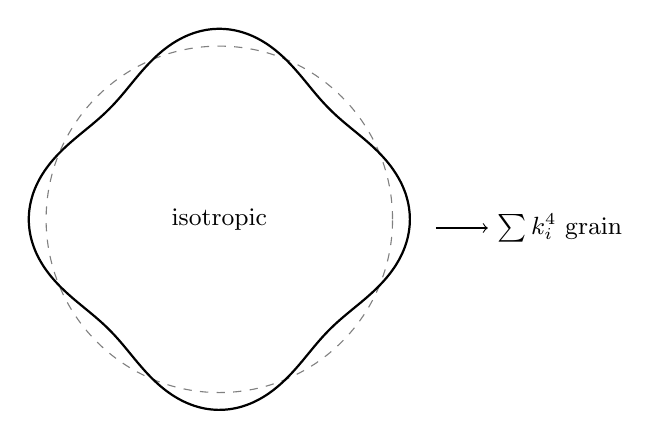
\begin{tikzpicture}[scale=2.2]
  \draw[gray, dashed] (0,0) circle (1);
  \draw[thick] plot[domain=0:360, samples=200, smooth]
    ({(1 + 0.10*cos(4*\x))*cos(\x)}, {(1 + 0.10*cos(4*\x))*sin(\x)});
  \node at (0,0) {\small isotropic};
  \draw[->] (1.25,-0.05) -- (1.55,-0.05) node[right] {\small $\sum k_i^4$ grain};
\end{tikzpicture}
\caption{Residual cubic anisotropy of the light cone on the cusp, exaggerated. The dashed circle is the isotropic cone. The solid curve adds the degree-four lattice term, giving a relative distortion of order $(E/E_{\mathrm{Planck}})^2$.}
\label{fig:cubic-aniso}
\end{figure}

The current dimension-six Lorentz-violation limits are weak, requiring only an effective scale above roughly $10^{-8}$ of the Planck scale, so a Planck-scale cusp anisotropy passes comfortably. The falsifier runs both ways. Measuring exact Lorentz invariance to arbitrarily high energy, with no anisotropy at the predicted scale, would kill the discrete substrate. Conversely, a lower effective cutoff would push $\delta$ up into the testable range. This is the sharpest experimental handle the model offers.

\subsection{What else would falsify it}

\begin{itemize}
  \item A fourth generation, or a clean failure of the running $\sin^2\theta_W$ and $b$-$\tau$ numbers.
  \item No low-energy supersymmetry anywhere, together with a measured $\sin^2\theta_W$ that bare Standard Model running cannot reach. This tension is taken up in the open-problems section.
  \item A demonstration that the rule supplies no stabilizer, so that matter would not form, overturning the measured Skyrme result.
\end{itemize}


The substrate is not a just-so story. It produces numbers, and it names its own executioner in the form of a cubic anisotropy at the Planck scale. The clear division between exactly derived ratios and computed-and-compared low-energy values is kept throughout, so the predictions are read for what they are.
